\section{主储存器}

\subsection{作业}

\begin{problem}
    习题 1
    \begin{solution}
        \begin{enumerate}
            \item[\textbf{1)}] 存取时间是储存器完成存取操作所需要的时间，存取周期是储存器的相邻两次存取操作间隔的最小时间。
            
            \item[\textbf{2)}] 储存期带宽只储存器在单位时间内能传输的数据总量。题目中储存器带宽为
            $$
            B = \frac{64 \,\mathrm{bit}}{2 \times 10^{-7} \,\mathrm{s}} = 3.2 \times 10^{8} \,\mathrm{bit / s} = 40 \,\mathrm{MB / s}
            $$
        \end{enumerate}
    \end{solution}
\end{problem}

\begin{problem}
    习题 2
    \begin{solution}
        每个字 $32$ 位，占 $4$ 字节，因此 $64 \,\mathrm{KB} = 2^{16} \,\mathrm{B}$ 包含了 $2^{14}$ 个字。因此寻址范围是 $0 \sim 16383$。

        主存字节地址 $A_{15} A_{14} \dots A_0$ 总共 $16$ 位，可以使用 $A_{15} A_{14} \dots A_2$ 编码字地址，$A_1 A_0$ 选择字内部的字节。
    \end{solution}
\end{problem}

\begin{problem}
    习题 3
    \begin{solution}
        \begin{enumerate}
            \item[\textbf{1)}] 地址线 $16$ 根，数据线 $32$ 根。
            \item[\textbf{2)}] 行选择线和列选择先各 $2^{8} = 256$ 条。
            \item[\textbf{3)}]\ 
            \begin{center}
                \begin{mytable}{ccccc}
                    芯片规格 & 字扩展倍数 & 位扩展倍数 & 芯片总数 & 排列方式 \\
                    $2\mathrm{K} \times 8$ & $32$ & $4$ & $128$ 片 & $32$ 组，每组 $4$ 片 \\
                    $4\mathrm{K} \times 4$ & $16$ & $8$ & $128$ 片 & $16$ 组，每组 $8$ 片 \\
                    $16\mathrm{K} \times 8$ & $4$ & $4$ & $16$ 片 & $4$ 组，每组 $4$ 片 \\
                    $4\mathrm{K} \times 32$ & $16$ & $1$ & $16$ 片 & $16$ 组，每组 $1$ 片 \\
                    $8\mathrm{K} \times 8$ & $8$ & $4$ & $32$ 片 & $8$ 组，每组 $4$ 片 \\
                \end{mytable}
            \end{center}
        \end{enumerate}
    \end{solution}
\end{problem}

\begin{problem}
    习题 4
    \begin{solution}
        \begin{enumerate}
            \item[\textbf{1)}] $256 \times 1024 = 262144$ 个字单元。
            \item[\textbf{2)}] $256 \times 1024 \times 8 = 2097152$ 个位元。
            \item[\textbf{3)}] 假设采用二维地址结构，行列均为 $2^{9}$，那么计数器需要 $9$ 位。
            \item[\textbf{4)}] 假设刷新周期为 $2\,\mathrm{ms}$，那么：
            
            \begin{center}
                \begin{mytable}{ccc}
                    刷新方式 & 相邻行刷新间隔 & 同一行刷新间隔 \\
                    集中刷新 & $0.25 \,\mathrm{\mu s}$ & $2 \,\mathrm{ms}$ \\
                    分散刷新 & $0.5 \,\mathrm{\mu s}$ & $256 \,\mathrm{\mu s}$ \\
                    异步刷新 & $\frac{2000}{512} \,\mathrm{\mu s}$ & $2 \,\mathrm{ms}$ \\
                \end{mytable}
            \end{center}
        \end{enumerate}
    \end{solution}
\end{problem}

\begin{problem}
    习题 5
    \begin{solution}
        每组由两片 $1\mathrm{K}\times4$ 位存储器并行连接，得到 $1\mathrm{K}\times8$ 位。每页含 $16$ 组，容量为 $16\mathrm{K}\times8$ 位；共用 $4$ 页即可得到 $64\mathrm{K}\times8$ 位，因此共需 $4\times16\times2=128$ 片存储器芯片。

        \begin{center}
            \begin{tikzpicture}[>=stealth, line width=0.55pt, font=\small]
                \tikzset{
                    decoder/.style={
                        draw, align=center,
                        minimum width=2.25cm,
                        minimum height=0.75cm
                    },
                    chip/.style={
                        draw, align=center,
                        minimum width=1.95cm,
                        minimum height=1.00cm
                    }
                }

                % 页译码和组译码
                \node[decoder] (page-dec) at (2.75,7.35) {$2\!:\!4$ 页译码器};
                \node[decoder] (group-dec) at (2.75,1.50) {$4\!:\!16$ 组译码器};

                \node[anchor=east] at (1.48,7.35) {$A_{15}\sim A_{14}$};
                \node[anchor=east] at (1.48,1.50) {$A_{13}\sim A_{10}$};

                \draw[->] (1.54,7.35) -- (page-dec.west);
                \draw[->] (1.54,1.50) -- (group-dec.west);

                % 四根独立的页选择信号 P_0,...,P_3
                \foreach \p/\port/\xx/\yy in {
                    0/7.58/4.55/6.10,
                    1/7.43/4.40/5.00,
                    2/7.28/4.25/3.90,
                    3/7.13/4.10/2.80}{
                    \draw[->] (3.88,\port) -- (\xx,\port) -- (\xx,\yy) -- (5.30,\yy);
                    \node[font=\scriptsize, above] at (4.94,\yy) {$P_{\p}$};
                }

                % 四个页面，每页16组，省略中间14组
                \foreach \p/\yy in {
                    0/6.10,1/5.00,2/3.90,3/2.80
                }{
                    \draw (5.30,\yy-0.43) rectangle (12.55,\yy+0.43);

                    \node at (5.95,\yy) {第\p 页};

                    \draw (6.75,\yy-0.29) rectangle (8.35,\yy+0.29);
                    \node[font=\footnotesize] at (7.55,\yy) {第0组};

                    \node at (9.36,\yy) {$\cdots$};

                    \draw (10.25,\yy-0.29) rectangle (11.95,\yy+0.29);
                    \node[font=\footnotesize] at (11.10,\yy) {第15组};

                    \draw[<-] (12.55,\yy) -- (13.20,\yy);
                }

                % 16根组选择线送往四个页面
                \draw (group-dec.east) -- (13.20,1.50) -- (13.20,6.10);

                \node[font=\scriptsize, above] at (10.30,1.50) {$G_0,\ldots,G_{15}$};

                % 总线宽度标记
                \draw (7.40,1.38) -- (7.58,1.62);
                \node[font=\scriptsize, above] at (7.49,1.62) {16};

                \node[font=\footnotesize] at (8.90,7.06) {每页 $16\times(1\mathrm{K}\times8)$};

                % 任意一组的内部结构
                \draw (3.35,-2.75) rectangle (13.20,0.42);
                \node[font=\footnotesize] at (8.38,0.13) {任意一组 $(p,g)$};

                % 两片1K×4芯片进行位扩展
                \node[chip] (low) at (6.65,-1.26) {$1\mathrm{K}\times4$\\低4位};

                \node[chip] (high) at (10.45,-1.26) {$1\mathrm{K}\times4$\\高4位};

                % 两片芯片共用低10位地址
                \draw (4.85,-0.42) -- (10.45,-0.42);
                \draw[->] (6.65,-0.42) -- (low.north);
                \draw[->] (10.45,-0.42) -- (high.north);

                \node[anchor=east, font=\footnotesize] at (4.76,-0.42) {$A_9\sim A_0$};

                % 两片芯片共用组片选信号
                \draw (4.85,-2.17) -- (10.45,-2.17);
                \draw[->] (6.65,-2.17) -- (low.south);
                \draw[->] (10.45,-2.17) -- (high.south);

                \node[anchor=east, font=\footnotesize] at (4.76,-2.17) {$P_p\land G_g$};

                % 两片分别连接数据总线的低4位和高4位
                \draw[->] (low.east) -- (7.95,-1.26);
                \node[anchor=west, font=\scriptsize] at (8.00,-1.26) {$D_3\sim D_0$};

                \draw[->] (high.east) -- (11.75,-1.26);
                \node[anchor=west, font=\scriptsize] at (11.80,-1.26) {$D_7\sim D_4$};
            \end{tikzpicture}
        \end{center}
    \end{solution}
\end{problem}

\begin{problem}
    习题 6
    \begin{solution}
        共有 $64 \times 2^{10} \times 16 = 2^{20} = 1048576$ 个储存基元。

        设芯片有 $a$ 根地址线，$d$ 根数据线，那么 $2^{a} d = 2^{20}$，因此 $d = 2^{20 - a}$。则 $a + d = a + 2^{20 - a}$，当 $a = 19, 20$ 时，有 $a + d$ 取最小值 $21$。因此地址线和数据线总和最小为 $21$ 根，共两种解答。
    \end{solution}
\end{problem}

\begin{problem}
    习题 7
    \begin{solution}
        \begin{enumerate}
            \item[\textbf{1)}] 最大主存空间为 $2^{16} \times 1 \,\mathrm{B} = 64 \,\mathrm{KiB}$。
            \item[\textbf{2)}] BIOS 区需要使用 ROM，用户程序区需要使用 RAM。共需要 2 张 ROM 和 6 张 RAM。
            \item[\textbf{3)}] 共 $8 = 2^{3}$ 张芯片，片选地址需要 $3$ 位，适合选择 74138 译码器。
        \end{enumerate}
    \end{solution}
\end{problem}

\begin{problem}
    习题 8
    \begin{solution}
        选择 $2$ 片 $4\mathrm{K}\times4$ 位 ROM 芯片进行位扩展，组成 $4\mathrm{K}\times8$ 位系统程序区；选择 $3$ 片 $4\mathrm{K}\times8$ 位 RAM 芯片组成 $12\mathrm{K}\times8$ 位用户程序区，共需要 $5$ 片芯片。系统程序区的地址为 $0000\mathrm{H}\sim0FFF\mathrm{H}$，用户程序区的地址为 $1000\mathrm{H}\sim3FFF\mathrm{H}$。

        连接图如下，图中带 \# 的控制信号均为低电平有效：

        \begin{center}
            \begin{tikzpicture}[x=1cm,y=1cm,line width=0.55pt,font=\footnotesize,every node/.style={inner sep=0.8pt}]
                \tikzset{mem/.style={draw,minimum width=3cm,minimum height=1.10cm,align=center,inner sep=2pt}}
                % 译码器和输入信号
                \draw (0.75,2.35) rectangle (3.35,10.15);
                \node[font=\small] at (2.05,9.68) {74LS138};
                \node at (2.05,3.55) {$G_1=1$};
                \foreach \y/\name/\pin in {9.02/{$A_{14}$}/C,8.28/{$A_{13}$}/B,7.54/{$A_{12}$}/A,6.55/{$\mathrm{MREQ}^{\#}$}/{$G_{2A}^{\#}$},5.55/{$A_{15}$}/{$G_{2B}^{\#}$}} {
                    \node[anchor=east] at (0.50,\y) {\name};
                    \draw (0.54,\y) -- (0.75,\y);
                    \node[anchor=west] at (0.89,\y) {\pin};
                }
                % 存储芯片：每片右侧仅在实际接线处与线相接
                \node[mem] at (7.55,9.65) {ROM1\\[-1pt]$4\mathrm{K}\times4$，$D_3\sim D_0$};
                \node[mem] at (7.55,8.00) {ROM2\\[-1pt]$4\mathrm{K}\times4$，$D_7\sim D_4$};
                \node[mem] at (7.55,6.35) {RAM1\\[-1pt]$4\mathrm{K}\times8$};
                \node[mem] at (7.55,4.70) {RAM2\\[-1pt]$4\mathrm{K}\times8$};
                \node[mem] at (7.55,3.05) {RAM3\\[-1pt]$4\mathrm{K}\times8$};
                % Y0 同时控制两片 ROM；Y1、Y2、Y3 分别控制三片 RAM
                \draw (3.35,8.825) -- (4.90,8.825);
                \draw (4.90,8.00) -- (4.90,9.65);
                \draw (4.90,9.65) -- (6.05,9.65);
                \draw (4.90,8.00) -- (6.05,8.00);
                \fill (4.90,8.825) circle (1.15pt);
                \node[anchor=south] at (3.84,8.93) {$Y_0^{\#}$};
                \foreach \i/\y in {1/6.35,2/4.70,3/3.05} {
                    \draw (3.35,\y) -- (6.05,\y);
                    \node[anchor=south] at (3.84,\y+0.10) {$Y_{\i}^{\#}$};
                }
                \node[font=\scriptsize] at (2.05,1.84) {$Y_4^{\#}\sim Y_7^{\#}$ 未使用};
                % 四根互相平行的公共线：地址线、数据线、读控制线、写控制线
                \foreach \x/\name in {9.95/{$A_{11}\sim A_0$},11.35/{$D_7\sim D_0$},12.75/{$\mathrm{OE}^{\#}$},14.15/{$\mathrm{WE}^{\#}$}} {
                    \draw (\x,2.18) -- (\x,10.26);
                    \node[anchor=south,font=\scriptsize] at (\x,10.43) {\name};
                }
                % 每片芯片的地址、数据、读控制连接；交叉处不加连接点
                \foreach \y in {9.65,8.00,6.35,4.70,3.05} {
                    \draw (9.05,\y+0.33) -- (9.95,\y+0.33); \fill (9.95,\y+0.33) circle (1.05pt);
                    \draw (9.05,\y+0.11) -- (11.35,\y+0.11); \fill (11.35,\y+0.11) circle (1.05pt);
                    \draw (9.05,\y-0.11) -- (12.75,\y-0.11); \fill (12.75,\y-0.11) circle (1.05pt);
                }
                % 仅三片 RAM 需要写控制线
                \foreach \y in {6.35,4.70,3.05} {
                    \draw (9.05,\y-0.33) -- (14.15,\y-0.33); \fill (14.15,\y-0.33) circle (1.05pt);
                }
            \end{tikzpicture}
        \end{center}

        图中的 $\mathrm{OE}^{\#}$、$\mathrm{WE}^{\#}$ 分别表示读控制信号和写控制信号：
        $$
        \mathrm{OE}^{\#}=\mathrm{MREQ}^{\#}\lor\neg(\mathrm{R/W}^{\#}),\qquad \mathrm{WE}^{\#}=\mathrm{MREQ}^{\#}\lor\mathrm{R/W}^{\#}.
        $$
    \end{solution}
\end{problem}


\begin{problem}
    习题 9
    \begin{solution}
        \begin{enumerate}
            \item[\textbf{1)}] 采用一片 74LS138 产生 $8$ 个片选信号，分别控制 $8$ 片 $8\mathrm{K}\times8$ 位 RAM。CPU 的 $A_{12}\sim A_0$ 接各片的地址端，$D_7\sim D_0$ 接各片的数据端，高三位地址 $A_{15}\sim A_{13}$ 接译码器。

            \begin{center}
                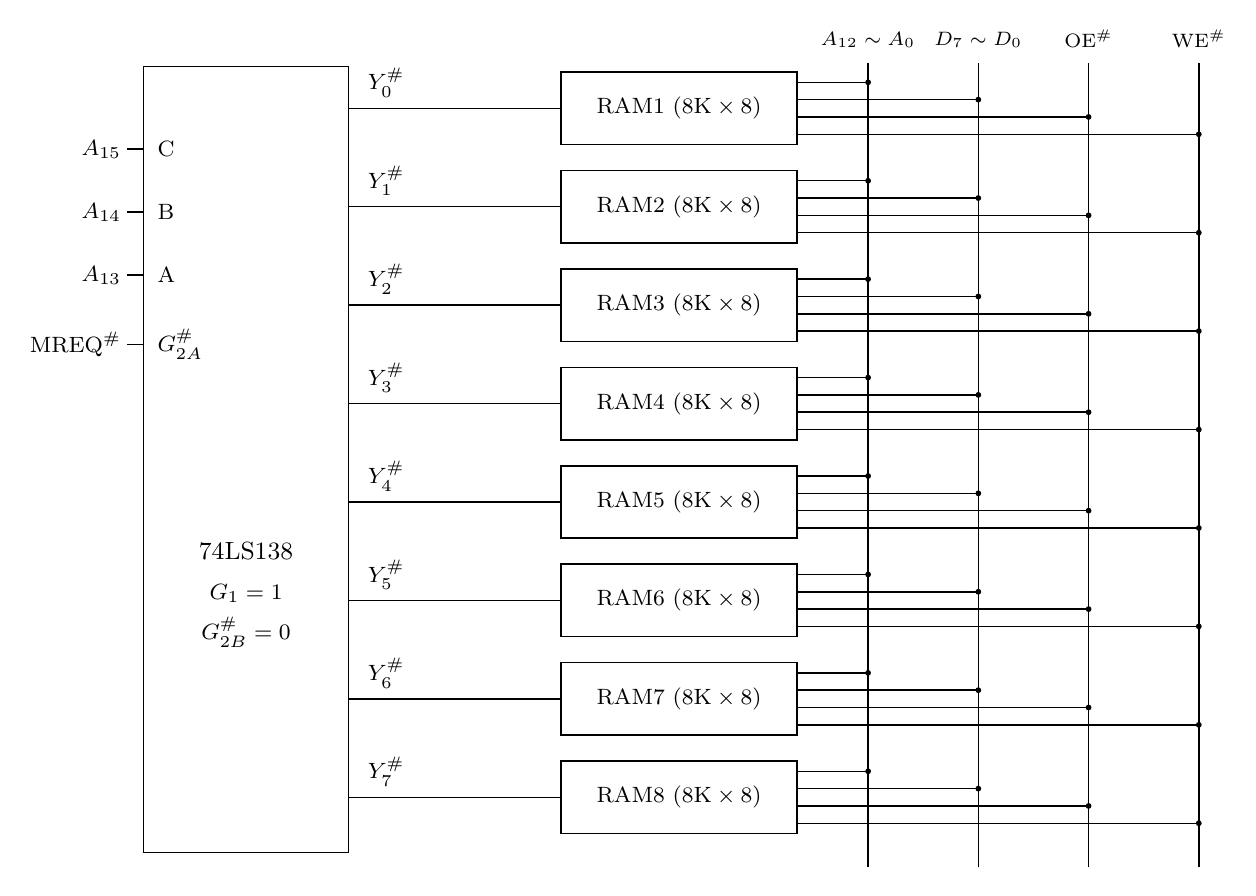
\begin{tikzpicture}[x=1cm,y=1cm,line width=0.55pt,font=\footnotesize,every node/.style={inner sep=0.8pt}]
                    \tikzset{mem/.style={draw,minimum width=3cm,minimum height=0.92cm,align=center,inner sep=2pt}}
                    % 译码器和输入信号
                    \draw (0.75,0.55) rectangle (3.35,10.53);
                    \node[font=\small] at (2.05,4.38) {74LS138};
                    \node at (2.05,3.84) {$G_1=1$};
                    \node at (2.05,3.35) {$G_{2B}^{\#}=0$};
                    \foreach \y/\name/\pin in {9.48/{$A_{15}$}/C,8.68/{$A_{14}$}/B,7.88/{$A_{13}$}/A,7.00/{$\mathrm{MREQ}^{\#}$}/{$G_{2A}^{\#}$}} {
                        \node[anchor=east] at (0.50,\y) {\name};
                        \draw (0.54,\y) -- (0.75,\y);
                        \node[anchor=west] at (0.89,\y) {\pin};
                    }
                    % 每条片选线直接连接对应芯片，同一行不拐弯
                    \foreach \num/\out/\y in {1/0/10.00,2/1/8.75,3/2/7.50,4/3/6.25,5/4/5.00,6/5/3.75,7/6/2.50,8/7/1.25} {
                        \node[mem] at (7.55,\y) {RAM\num\ $(8\mathrm{K}\times8)$};
                        \draw (3.35,\y) -- (6.05,\y);
                        \node[anchor=south] at (3.83,\y+0.10) {$Y_{\out}^{\#}$};
                    }
                    % 四根平行的公共线
                    \foreach \x/\name in {9.95/{$A_{12}\sim A_0$},11.35/{$D_7\sim D_0$},12.75/{$\mathrm{OE}^{\#}$},14.15/{$\mathrm{WE}^{\#}$}} {
                        \draw (\x,0.36) -- (\x,10.57);
                        \node[anchor=south,font=\scriptsize] at (\x,10.73) {\name};
                    }
                    % 所有 RAM 都接地址、数据、读、写控制
                    \foreach \y in {10.00,8.75,7.50,6.25,5.00,3.75,2.50,1.25} {
                        \draw (9.05,\y+0.33) -- (9.95,\y+0.33); \fill (9.95,\y+0.33) circle (1.05pt);
                        \draw (9.05,\y+0.11) -- (11.35,\y+0.11); \fill (11.35,\y+0.11) circle (1.05pt);
                        \draw (9.05,\y-0.11) -- (12.75,\y-0.11); \fill (12.75,\y-0.11) circle (1.05pt);
                        \draw (9.05,\y-0.33) -- (14.15,\y-0.33); \fill (14.15,\y-0.33) circle (1.05pt);
                    }
                \end{tikzpicture}
            \end{center}

            \item[\textbf{2)}] $8$ 片 RAM 的地址范围分别为
            $$
            \begin{aligned}
                &\text{RAM1}:\ \mathrm{0000H\sim1FFFH}, &&\text{RAM2}:\ \mathrm{2000H\sim3FFFH},\\
                &\text{RAM3}:\ \mathrm{4000H\sim5FFFH}, &&\text{RAM4}:\ \mathrm{6000H\sim7FFFH},\\
                &\text{RAM5}:\ \mathrm{8000H\sim9FFFH}, &&\text{RAM6}:\ \mathrm{A000H\sim BFFFH},\\
                &\text{RAM7}:\ \mathrm{C000H\sim DFFFH}, &&\text{RAM8}:\ \mathrm{E000H\sim FFFFH}.
            \end{aligned}
            $$

            \item[\textbf{3)}] $\mathrm{A000H}\sim\mathrm{BFFFH}$ 对应 RAM6。若 RAM6 的片选端被错误地一直保持为低电平，则写入其他 RAM 时，RAM6 也会同时被选中，导致 RAM6 的对应位置就会写入相同的数据。

            \item[\textbf{4)}] 若地址线 $A_{13}$ 与 CPU 断开后接到高电平，译码器输入端 $A$ 将一直为 $1$，因此只有 $Y_1^{\#}$、$Y_3^{\#}$、$Y_5^{\#}$、$Y_7^{\#}$ 可能有效。此时只能选中 RAM2、RAM4、RAM6、RAM8，其余四片不能被选中。
        \end{enumerate}
    \end{solution}
\end{problem}